\chapter{premier chapitre}
\label{chap:chap_1}

\section{exemples de base}
\label{sec:sec_examples_chap_1}

\subsection{listes}
\label{subsec:subsec_list}

\begin{enumerate}
  \item {\bf Premier point (gras) ;}
  \item {\em Second point (italique) ;}
  \item {\Large Troisième point (gros) ;}
      \begin{enumerate}
          \item {\small Premier sous-point en petit}
          \item {\tiny Second sous-point (petit)}
          \item {\Huge Troisième sous-point (très gros)}
      \end{enumerate}
  \item[$\bullet$] {\sf Point avec une puce (sans serif)}
  \item[$\circ$] {\sc Point avec un autre style de puce (petites lettres capitales)}
\end{enumerate}

\subsection{citations}

Ceci est un premier exemple de citation standard \cite{RN3}. Vous pouvez ensuite forcer l'utilisation des citation entre parenthèse pour le format APA-Provost tel que, \citep{RN4}. Enfin, vous pouvez également citer les auteurs \citet{RN5} de cette manière, ou ne citer que l'année de publication en  \citeyear{RN5}.

\subsection{liens}

Si vous utilisez \href{https://code.visualstudio.com/}{Visual Studio Code} pour composer votre document \LaTeX{}, vous pouvez utiliser l'extension \textit{vscode-ltex} disponible \textit{via} le lien suivant : \url{https://github.com/valentjn/vscode-ltex} pour corriger vos erreurs d'orthographe et de grammaire.

\subsection{notes de bas de page}

Vous pouvez utiliser les notes de bas de page pour inclure un lien\footnote{\url{https://www.uqac.ca}} en rapport avec votre texte, ou pour donner plus de précisions\footnote{Cette note de bas de page propose plus d'informations}.

\subsection{acronymes}

Exemple de définition d'un acronyme de trois lettres : \ac{TLA}. Puis utilisation de cet acronyme en version courte \acs{TLA}. Vous pouvez également mettre au pluriel l'acronyme long tel que, \aclp{TLA} ainsi que l'acronyme court : \acsp{TLA}.

\subsection{figures}

\begin{figure}[H]
 \centering
 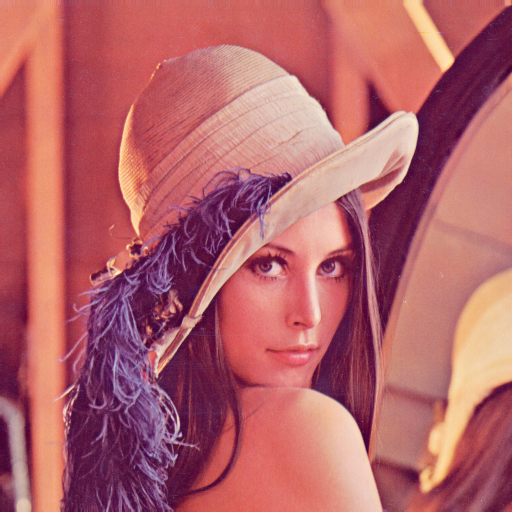
\includegraphics[width=7cm]{lenna.png}
 \caption{Titre de la figure qui doit normalement se tenir sur deux lignes dans la liste des figures.}
 \label{fig:figure_long}
\end{figure}

Vous pouvez ensuite mentionner la Figure \ref{fig:figure_long} dans votre texte.

\begin{figure}[H]
  \centering
  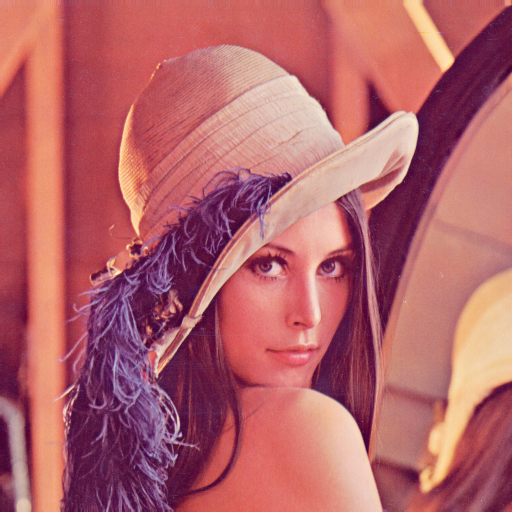
\includegraphics[width=7cm]{lenna.png}
  \caption[Titre de la figure sans citation]{Titre de la figure qui comporte une citation de \citet{RN6}.}
  \label{fig:figure_cite}
 \end{figure}

 Vous pouvez aussi référencer la Figure \ref{fig:figure_cite} directement dans votre texte.

\subsection{tableaux}

\begin{table}[H]
  \begin{center}
    \caption{Titre du tableau qui doit normalement se tenir sur deux lignes dans la liste des tableaux.}
    \label{tab:tab_1}
    \begin{tabular}{l|c|r}
      \textbf{Value 1} & \textbf{Value 2} & \textbf{Value 3}\\
      $\alpha$ & $\beta$ & $\gamma$ \\
      \hline
      1 & 1110.1 & a\\
      2 & 10.1 & b\\
      3 & 23.113231 & c\\
    \end{tabular}
  \end{center}
\end{table}

Vous pouvez ensuite mentionner le Tableau \ref{tab:tab_1} dans votre texte.
